%% Submissions for peer-review must enable line-numbering
%% using the lineno option in the \documentclass command.
%%
%% Preprints and camera-ready submissions do not need
%% line numbers, and should have this option removed.
%%
%% Please note that the line numbering option requires
%% version 1.1 or newer of the wlpeerj.cls file, and
%% the corresponding author info requires v1.2

\documentclass[fleqn,10pt,lineno]{wlpeerj} % for journal submissions
% \documentclass[fleqn,10pt]{wlpeerj} % for preprint submissions
\usepackage{textcomp} %for \textgreater
\usepackage{wasysym} %for \times
\usepackage{hyperref}

\title{Patterned progression of gut microbiota predisposes preterm infants to necrotizing enterocolitis and late onset sepsis: prospective pilot data from a non-Western population}

\author[1]{Jiayi Liu}
\author[2]{Jianhua Sun}
\author[3]{Yuqing Li}
\author[4]{Yi Feng}
\author[5]{Liya Pan}
\author[6]{Zhoulonglong Xie}
\author[7]{Zhilong Yan}
\author[8]{Jianhua Zhao}
\author[9]{Li Hong}


\affil[1]{Department of Clinical Nutrition, Shanghai Children's Medical Center, School of Medicine Shanghai Jiao Tong University, Shanghai, China}
\affil[2]{Department of Clinical Nutrition, Shanghai Children's Medical Center, School of Medicine Shanghai Jiao Tong University, Shanghai, China}
\affil[3]{Department of Clinical Nutrition, Shanghai Children's Medical Center, School of Medicine Shanghai Jiao Tong University, Shanghai, China}
\affil[4]{Department of Clinical Nutrition, Shanghai Children's Medical Center, School of Medicine Shanghai Jiao Tong University, Shanghai, China}
\affil[5]{Department of Clinical Nutrition, Shanghai Children's Medical Center, School of Medicine Shanghai Jiao Tong University, Shanghai, China}
\affil[6]{Department of Clinical Nutrition, Shanghai Children's Medical Center, School of Medicine Shanghai Jiao Tong University, Shanghai, China}
\affil[7]{Department of Clinical Nutrition, Shanghai Children's Medical Center, School of Medicine Shanghai Jiao Tong University, Shanghai, China}
\affil[8]{Shanghai Majorbio Bio-Pharm Technology Co., Ltd, Shanghai, China}
\affil[9]{Department of Clinical Nutrition, Shanghai Children's Medical Center, School of Medicine Shanghai Jiao Tong University, Shanghai, China}
\corrauthor[9]{Li Hong}{hongli@scmc.com.cn}

%\keywords{Gut Microbiota, Preterm Infant, Necrotizing Enterocolitis, Neonatal Late Onset Sepsis, High Throughput DNA Sequencing, DADA2}

\begin{abstract}
\textbf{Background and Objectives} \\Intestinal microbiota dysbiosis might predispose preterm infants to necrotizing enterocolitis(NEC) and late onset sepsis(LOS). In this observational prospective study, we aimed to profile and compare postpartum microbiota progression patterns in non-Western preterm patients with either condition. \\
\textbf{Methods} \\We enrolled preterm infants with gestational age less than 33 weeks and birth weight more than 950g, from July 2013 to December 2014. We began fecal sample collection from the the first stool after birth and prospectively collected until discharge. Bacterial V3~V4 region of 16s rRNA genes from each stool sample were amplified and sequenced. With the use of RM two-way ANOVA and Zero-Inflated Beta Random Effect models to account for repeated measures, we found out the development of NEC or LOS associated with gut bacterial communities. \\
\textbf{Results}\\A total of 192 fecal samples from 24 patiens were studied, of whom four developed NEC, three LOS; the remaining 17 were used as controls. [The post-partum gut microbiota colonization started to diverge among NEC, LOS and their matched control groups, from the second week after birth.  Microbiota of the LOS infants was the least diversified (Shannon index=1.66), while that of the control group was the most diversified(Shannon index=0.88, p=0.01). Potentially pathogenic genus Enterococcus (20.86\%) and Staphylococcus (8.67\%) were prominent in NEC patients and Klebsiella (42.15\%) in LOS group. Both two groups addressed lower proportion of Lactococcus (7.98\% and 13.76\% in NEC and LOS group, respectively) than the control group (3.66\%)].\\

%The microbial community structure in case stools diff ered signifi cantly from those in control stools. These diff erences emerged only after the fi rst month of age. In mixed models, the time- by-necrotising-enterocolitis interaction was positively associated with Gammaproteobacteria (p=0·0010) and negatively associated with strictly anaerobic bacteria, especially Negativicutes (p=0·0019). We studied 1094 stool samples from 44 infants in the secondary cohorts. 18 infants developed necrotising enterocolitis (cases) and 26 were controls. After combining data from all cohorts (166 infants, 3586 stools, 46 cases of necrotising enterocolitis), there were increased proportions of Gammaproteobacteria (p=0·0011) and lower proportions of both Negativicutes (p=0·0013) and the combined Clostridia–Negativicutes class (p=0·0051) in infants who went on to develop necrotising enterocolitis compared with controls. These associations were strongest in both the primary cohort and the overall cohort for infants born at less than 27 weeks’ gestation.

\textbf{Conclusions}\\Postpartum colonization pattern of gut microbiome might predispose preterm newborns to NEC or LOS, in which reduced diversity of the whole microbiota community and potentially pathogenic genus could have played an essential role in disease progression. Still, more studies are needed to identify etiological strains, underlying mechanisms and correspondent microbial patterns.
\end{abstract}

\begin{document}

\flushbottom
\maketitle
\thispagestyle{empty}

\section*{Introduction}
%intro gutmicrobiota, its role in health, early pattern a/w disease
Gut microbiota is a key contributor to human health and the dysbiosis of which are proven to be associated with multiple diseases, such as atherosclerosis\citep{tang2017gut}, obesity\citep{bouter2017role}, neuropathy\citep{sarkar2016psychobiotics}, liver diseases\citep{tilg2016gut}, etc. Temporal colonization pattern of the intestinal microbiota during early stages of life\cite{} also provided evidence of its association with early life events, including Type 1 diabetes\citep{giongo2011toward, vatanen2018human}, asthma\citep{stokholm2018maturation} and allergy\citep{madan2012normal,savage2018prospective}. In light of less gut maturity, innate immunity and more C-setions birth modes, microbiome assembly in pretem infants often differs from that of term infants,  especially presenting with lower \textit{Bifidobacterium} spp. abundance and higher \textit{Escherichia coli}, \textit{Enterococcus} sp., and \textit{Klebsiella pneumoniae}\citep{schwiertz2003development, bezirtzoglou2011microbiota}. As as result, perturbation of postpartum microbiota haboring contributes to the vulnerablilty in preterm-associated health consequencese, such as necrotizing enterocolitis and late-onset sepsis.

%intro gutmicrobiota, its role in health, early pattern a/w Necrotizing

\noindent
Necrotizing enterocolitis, characterized by rapid progression, high morbidity and mortality, is one of the most devastating gestrointestinal neonatal emergencies, especially in preterm newborns; the etiologies of which remains elusive. Previous studies have suggested how intestinal microbiota pattern is implicated in the condition. Mai et al. reported an increase in the Proteobacteria and a decrease in the Firmicutes phyla during three to seven days prior to NEC onset (Mai et al., 2011). Zhou et al. reported a relatively higher abundance of Clostridium and Gamma-Proteobacteria in the proximity of NEC during early and late onset, respectively\citep{zhou2015longitudinal}. Dominance of \citep{Citrobacter koseri} and/or Klebsiella pneumoniae was found to correlate with NEC risk in preterm infants

\

\noindent
 Among non-Western population, however, microbiota chronological dysbiosis preceding necrotizing enterocolitis or late onset sepsis remain scant so far. Hence, we conducted this prospective study with the aims to profile and compare post-postpartum pattern of intestinal microbiota in Chinese preterm infants who subsequently developed necrotizing enterocolitis and late onset sepsis, which may be critical in the etiopathogenesis of disease.

\section*{Methods}
  \subsection*{Ethics}
  This study was approved by the joint committee of ethics of Shanghai Children’s Medical Center, School of Medicine Shanghai Jiao Tong University (SCMCIRB-K2013022). Detailed written informed consent was obtained from the parents prior to fecal sample collection.

  \subsection*{Patients}
  Newly born preterm infants with gestational age less than 33 weeks, birth weight over 950g were enrolled from Neonatal Intensive Care Unit at Shanghai Children’s Medical Center from July 2013 to December 2014. The exclusion criteria were 1) diagnosed with early-onset sepsis, 2) hepatic diseases, 3) renal impairment (Cr \textgreater 88 $\mu$M), 4) diagnosed with intestinal obstruction, 5) in foreseeable need of cardiovascular or abdominal surgeries (except for male circumcision or PDA ligation), 6) estimated parenteral support to supply over 50\% of daily caloric intake for more than four days, 7) given intravenous antibiotics administration (except prophylactic regimen of cefotaxime, piperacillin-tazobactam and/or metronidazole), 8) history of oral antibiotics administration, 9) grossly bloody stools at admission, and 10) over five days old.

  \noindent
  NEC cases were defined as infants who met the criteria for Stage II and Stage III NEC disgnosis\citep{bell1978neonatal}, including radiographic intestinal dilation, ileus, pneumatosis intestinalis, and/or absent bowel sounds with or without abdominal tenderness, and/or mild metabolic acidosis and thrombocytopenia. LOS cases was diagnosed if 1)an infant had a positive hemoculture or other suspicious loci of infection after 72 hours of life, with septic signs/symptoms reviewed independently by at least two neonatologists, and had been treated with advanced antibiotics (e.g., Meropenem) after diagnosis. Infants with no infectious complications or sepsis were regarded as controls.

  \subsection*{Sample collection and handling}
  Fecal samples collection began from neonatal meconium till discharge. Although we intended to collect fecal samples on a daily basis, due to working shifts and flexible clinical scheduling, we set seven days as the maximum interval between two collections from every infant. Every sample was collected within 30 minutes of defecation from infants' diaper with a sterile spatula. The samples were immediately placed in a cryogenic vial on dry ice and stored at 80\textdegree{}C within 30 minutes without additives. All samples were collected and stored before knowing the diagnosis of respective patients.

  \subsection*{DNA extraction and quality control amplification and 16s rRNA gene sequencing}
  Microbial genomic DNA was isolated from each fecal specimen using the E.Z.N.A.® Soil DNA Kit (Omega Bio-Tek, Norcross, GA, U.S.) according to manufacturer’s protocols. The concentration and purity of the DNA were determined by NanoDrop 2000 UV-vis spectrophotometer (Thermo Scientific, Wilmington, USA), and the DNA quality was checked by 1\% agarose gel electrophoresis.

  \subsection*{Broad-range PCR and High-throuput Sequencing of 16s rRNA gene amplicons}
  The V3-V4 hypervariable regions of the bacterial 16S rRNA gene were amplified from each sample using bacterial\/archaeal primers 338F (5’-ACTCCTACGGGAGGCAGCAG-3’) and 806R (5’-GGACTACHVGG GTWTCTAAT-3’) using thermocycler PCR system (GeneAmp 9700, ABI, USA). The PCR reactions were as follows: 3 min of denaturation at 95 °C, 27 cycles of 30 s at 95 °C, 30 s annealing at 55 °C and 45 s elongation at 72 °C, and a final extension at 72 °C for 10 min. The PCR reactions were performed in triplicate, with each 20 $\mu$L mixture containing 4 $\mu$L 5X FastPfu Buffer, 2 $\mu$L 2.5 mM dNTPs, 0.8 $\mu$L of each primer (5 $\mu$M), 0.4 $\mu$L FastPfu Polymerase and 10 ng template DNA. The PCR products were extracted from a 2\% agarose gel and further purified using the AxyPrep DNA Gel Extraction Kit (Axygen Biosciences, Union City, CA, USA), and quantified using QuantiFluor™-ST (Promega, USA) according to the manufacturer’s protocols.

  \noindent
  Equimolar amounts of purified amplicons were pooled and paired\-end sequenced (2 x 300) on an Illumina MiSeq platform (Illumina, San Diego, USA) according to the standard protocols of Majorbio Bio-Pharm Technology Co. Ltd. (Shanghai, China). The reads were de-multiplexed using the Illumina software and separate FASTQ files were generated for each specimen and deposited to the Sequence Read Archive NCBI under the BioProject accession PRJNA470548. Another public archive repository is available at \href{https://figshare.com/articles/Untitled_Item192_samples_for_publishing_Longitudinal_gut_microbiota_patterns_in_preterm_infants_with_necrotizing_enterocolitis_or_late-onset_sepsis_an_observational_prospective_study_/7205102}{figshare doi: 10.6084/m9.figshare.7205102}

  \subsection*{Raw Data Processing}
  After pyrosequencing, de-multiplexed sequence reads were subjected to quality filtering utilizing Trimmomatic software(version????)\citep{bolger2014trimmomatic},  and were truncated at any site with an Phred score \textless 20 over a 50bp-sized window; barcode matching with the primer mismatch from 0 to 2 nucleotides was adopted and reads containing ambiguous characters were removed. After trimming, FLASh(Fast Length Adjustment of Short Read)\citep{magovc2011flash}, a read pre-processing software, assembled and merged the paired-end reads from fragments and generated \textgreater 10 bp overlapped, with the dead match ratio 0.2. Unassembled reads were discarded.

  \noindent
  To fairly compare all the samples at the same sequencing depth, the "sub.sample" command of mothur program(version1.30.1)\citep{schloss2009introducing} was used for normalization to the smallest sample size. \href{https://www.drive5.com/usearch/manual/uchime_algo.html}{UCHIME Algorithm} detected chimeric sequences, removed chimera to obtain effective reads, which were then sorted by cluster size and processed using Operational Taxonomic Units(OTUs) with 97\% similarity cutoff using \href{http://drive5.com/uparse/}{USEARCH v7}(UPARSE version 7.1). The taxonomy of each 16S rRNA gene sequence was analyzed by \href{http://rdp.cme.msu.edu/}{RDP Classifier algorithm}\citep{wang2007naive} against the Silva (SSU128)\citep{quast2012silva} 16S rRNA database using confidence threshold of 70\%. Each sequence was assigned the taxonomy by QIIME\citep{caporaso2010qiime}. The representative sequences were allocated phylogenetically down to the domain, phylum, class, order, family, and genus levels. The relative abundance of a given taxonomic group was calculated as a percentage of the sequences number belonging to that group devided by the total number of obtained sequences.

  \noindent
   Within-sample diversity(alpha diversty) analysis, including Shannon index and Observed species richness (sobs), were obtained using the "summary.single" command of mothur program(version1.30.1)\citep{schloss2009introducing}. Between-sample diversity(beta diversity) analysis was obtained estimating weighted UniFrac distances between samples.

  \subsection*{Statistical and Bioinformatics Analysis}
    \subsubsection*{Demographics and Clinical Sample comparisons}
    Kruskal-Wallis test and Wilcoxon rank-sum test were used to identify statistically significant differences in continuous variables ,including gestational age, birth weight, age when the patients were diagnosed and length of hospitilisation. The $\chi^2$, or Fisher's exact test were used to identify differences in gender composition. $\alpha$ level was considered 0.05 for all statistical tests . All statistical test not involving microbiome 16s rRNA sequencing data was performed using \textit{"stats"} package using R(v.3.5.1).
    \subsubsection*{Microbiota and Bioinformatics Analyses}
      \paragraph{Diversity Analyses}
      $\alpha$ diversity
      \paragraph*{Disease-related Time Interval Determination}
      Under the circumstance that the sampling and disease onset timepoints for each patient were not perfectly universal, to illustrated the continuous longitudinal and repeated nature of the sampling and its relationship with onset and progression of diseases, we seperated the whole sampling span into 7 time intervals:
        \begin{enumerate}[noitemsep]
          \item early post-partum(EPP): within 3 days afterbirth
          \item early pre-onset(EPO): from the end of EPP to at least four days befor disease onset
          \item late pre-onset(LPO): from the end of EPO to the start of onset
          \item early disease: first third interval of whole disease span
          \item middle disease: second third interval of whole disease span
          \item late disease: last third interval of whole disease span
          \item post disease: from the end of disease to discharge timepoint
        \end{enumerate}
      \paragraph*{Modeling Strategies}
      To compare the dynamics of microbiota diversity and relative taxonomic abundance preciding the disease, we took into account the EPP, EPO, LPO and ED interval among all patients and fit(Summlemantary matrix1).
      To compare the microbiome profile right after birth until disease alleviation, we selected EPP, EPO, LPO, ED, MD and LD interval of NEC and LOS patients(Supplementary matrix2).
      The average value of diversity indexes and relative abundances, if more than two were available within one analysis interval, of each patient was calculated.
      Zero-Inflated Beta Regression Model with Random Effects (ZIBR) and Linear Mixed-effects Model(LME) were used to test the association between OTU relative abundance and clinical covariates (diseases-related time intervals) for longitudinal microbiome data \citep{chen2016two}. \textit{ZIBR} package were utilized for modeling.

      \noindent
      \textit{ZIBR} package were utilized for modeling. Figures were generated with the \textit{"ggpubr"}\citep{kassambara2017ggpubr} and \textit{"ggplot2"}\citep{ggplot2} packages using R(v.3.5.1).
      Scripts for modeling and figures plotting, input and output files, figures are available at our \href{https://github.com/jiayiliujiayi/NEC-LOS-microbiota_pattern_comparison}{github repository}.

    \subsubsection*{Scripts and Figures Archiving}
    Figures were generated with the \textit{"ggpubr"}\citep{kassambara2017ggpubr} and \textit{"ggplot2"}\citep{ggplot2} packages using R(v.3.5.1)

\section*{Results}
  A total of 7,472,400 optimized V3-V4 tags of 16s rRNA gene sequences were produced from 192 fecal samples, with an average length of 448 bp.(Table S1)
  \subsection*{Patients characteristics}
   Totally 130 infants met the criteria of our study, and 1698 samples were collected from them in the neonatal intensive care unit (NICU) at Shanghai Children’s Medical Center from July 2013 to December 2014.  Among whom, we studied 192 fecal samples from 24 well-sampled preterm infants, including four subsequently diagnosed with NEC (2 in stage IIA and 2 in stage IIB), three with LOS, and 17 matched controls (Figure\ref{fig:design} ,Table S2). Fecal samples were collected between days 1 and 69 of life. Sampling timepoints and numbers of samples varied among each infant.
     \begin{figure}[ht]\centering
       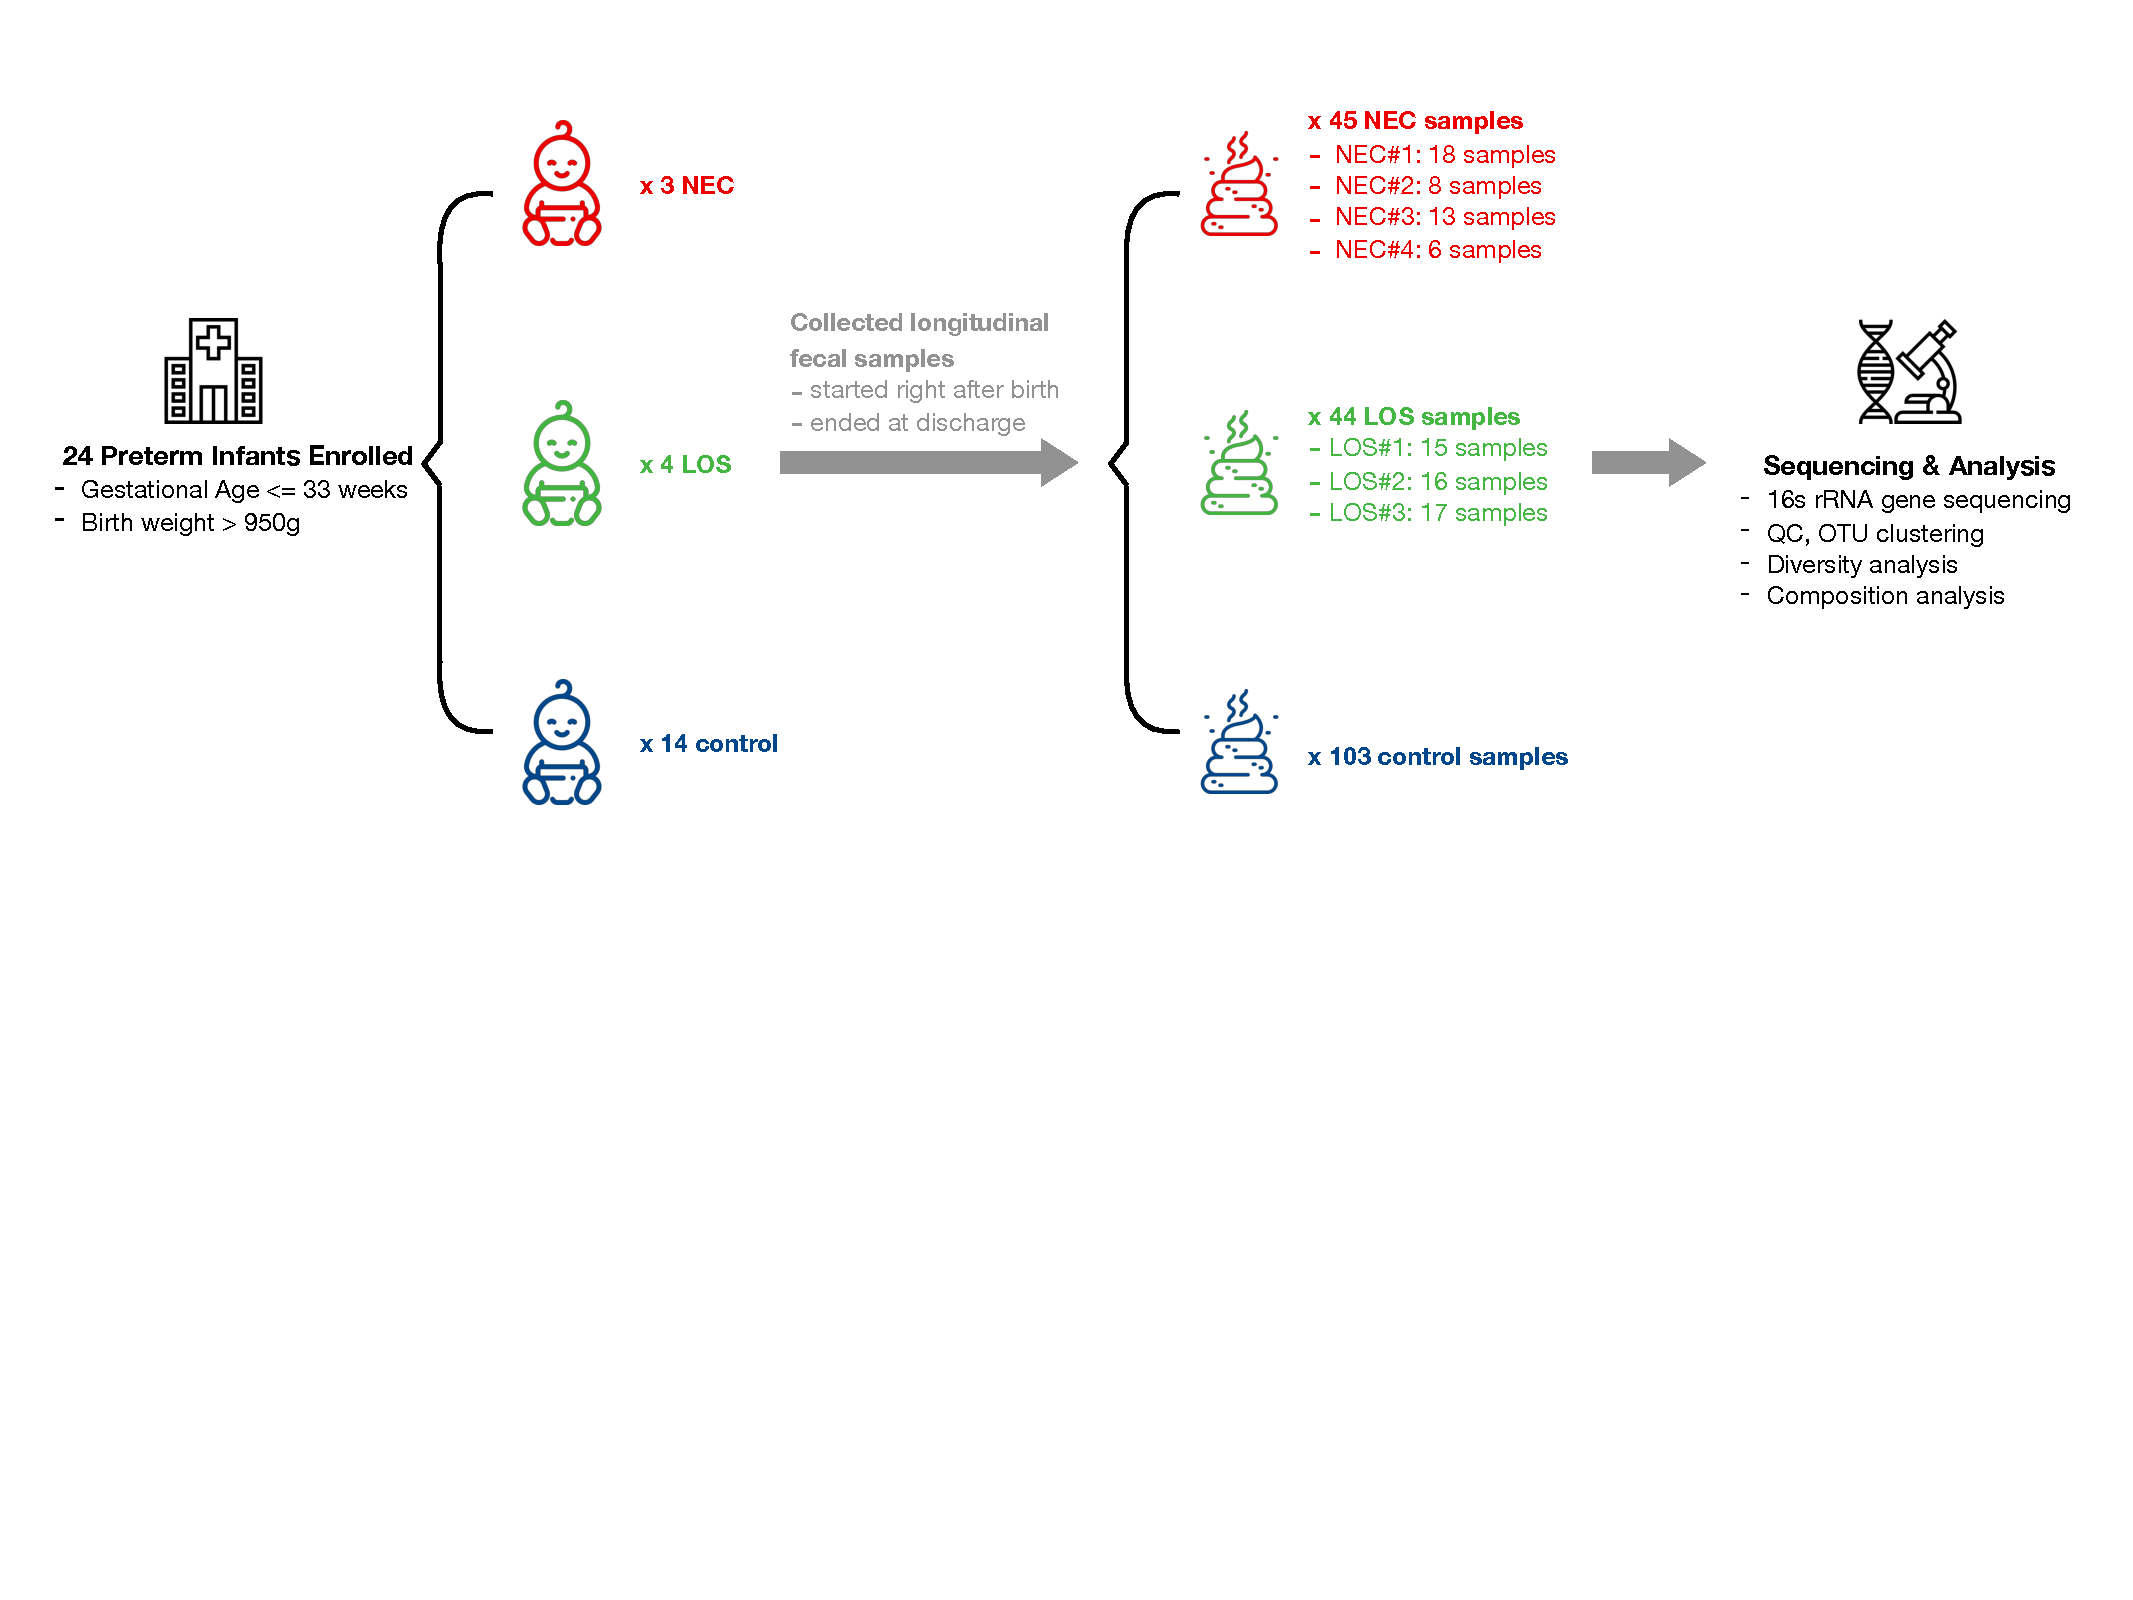
\includegraphics[width=\linewidth]{figure/design.pdf}
       \caption{Flow of Study Design}
       \label{fig:design}
     \end{figure}

  \noindent
   All infants were delivered by cesarean section and fed on infant formula. No one was prescribed probiotics during hospitalization. Comparisons showed no significant difference in terms of gestational age, birth weight and gender proportions, diagnosed age among three groups (Table 1). Lenth of stay mong three groups was significantly different however rational since NEC and LOS patients usually require longer period of healthcare because of there worse conditions compared with the control group.
   All infants were delivered by cesarean section and fed on infant formula. No one was prescribed probiotics during hospitalization.

   \subsection*{Microbiota Diversity}

\section*{Discussion}
are consistent with the hypothesis that dysbiosis precedes this severe event. The

\noindent
Our study has its limitations. We acknowledge that the sample size is limited since this study is single-center-based and the incidence of both diseases are relatively low: among the 1148 preterm infants admitted within July 2013 to December 2014, only five developed NEC. Furthermore, the resultant overfitting possibility inevitably rose up, which became the pitfall in understanding the true microbiota patterns preceding NEC and LOS.

\section*{Conclusions}
Necrotizing enterocolitis, a worldwidely concern that threatern


\section*{Acknowledgments}
We appreciate the support from enrolled patients, their families, and all staffs at Shanghai Children’s Medical Center.


%microbiota development in infancy, sequence effect, Conversely, adequate maturation of the gut microbiome in this period may protect these pre-disposed children.
%increase vulnerability

%"#00468BB2" "#ED0000B2" "#42B540B2"




\section*{Some \LaTeX{} Examples}
\label{sec:examples}

Use section and subsection commands to organize your document. \LaTeX{} handles all the formatting and numbering automatically. Use ref and label commands for cross-references.

\subsection*{Figures and Tables}

Use the table and tabular commands for basic tables --- see Table~\ref{tab:widgets}, for example. You can upload a figure (JPEG, PNG or PDF) using the project menu. To include it in your document, use the includegraphics command as in the code for Figure~\ref{fig:view} below.

\begin{figure}[ht]
\centering

\includegraphics[width=\linewidth]{view.jpg}
\caption{An example image.}
\label{fig:view}
\end{figure}

\begin{table}[ht]
\centering
\begin{tabular}{l|r}
Item & Quantity \\\hline
Widgets & 42 \\
Gadgets & 13
\end{tabular}
\caption{\label{tab:widgets}An example table.}
\end{table}

\subsection*{Citations}

LaTeX formats citations and references automatically using the bibliography records in your .bib file, which you can edit via the project menu. Use the cite command for an inline citation, like \cite{Figueredo:2009dg}, and the citep command for a citation in parentheses \citep{Figueredo:2009dg}.

\subsection*{Mathematics}

\LaTeX{} is great at typesetting mathematics. Let $X_1, X_2, \ldots, X_n$ be a sequence of independent and identically distributed random variables with $\text{E}[X_i] = \mu$ and $\text{Var}[X_i] = \sigma^2 < \infty$, and let
$$S_n = \frac{X_1 + X_2 + \cdots + X_n}{n}
      = \frac{1}{n}\sum_{i}^{n} X_i$$
denote their mean. Then as $n$ approaches infinity, the random variables $\sqrt{n}(S_n - \mu)$ converge in distribution to a normal $\mathcal{N}(0, \sigma^2)$.

\subsection*{Lists}

You can make lists with automatic numbering \dots

\begin{enumerate}[noitemsep]
\item Like this,
\item and like this.
\end{enumerate}
\dots or bullet points \dots
\begin{itemize}[noitemsep]
\item Like this,
\item and like this.
\end{itemize}
\dots or with words and descriptions \dots
\begin{description}
\item[Word] Definition
\item[Concept] Explanation
\item[Idea] Text
\end{description}

We hope you find write\LaTeX\ useful for your PeerJ submission, and please let us know if you have any feedback. Further examples with dummy text are included in the following pages.

\section*{Methods}

\lipsum[4] % Dummy text

\begin{equation}
\cos^3 \theta =\frac{1}{4}\cos\theta+\frac{3}{4}\cos 3\theta
\label{eq:refname2}
\end{equation}

\lipsum[5] % Dummy text

\subsection*{Subsection}

\lipsum[6] % Dummy text

\paragraph{Paragraph} \lipsum[7] % Dummy text
\paragraph{Paragraph} \lipsum[8] % Dummy text

\subsection*{Subsection}

\lipsum[9] % Dummy text

\begin{figure}[ht]\centering
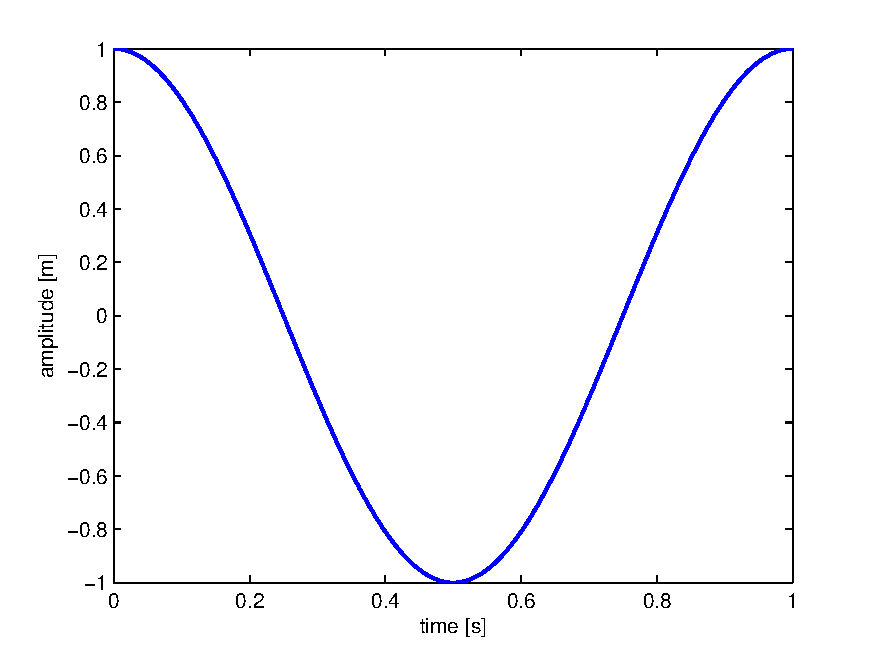
\includegraphics[width=\linewidth]{results}
\caption{In-text Picture}
\label{fig:results}
\end{figure}

Reference to Figure \ref{fig:results}.

\section*{Results and Discussion}

\lipsum[10] % Dummy text

\subsection*{Subsection}

\lipsum[11] % Dummy text

\subsubsection*{Subsubsection}

\lipsum[12] % Dummy text

\subsubsection*{Subsubsection}

\lipsum[14] % Dummy text

\subsection*{Subsection}

\lipsum[15-20] % Dummy text

\section*{Acknowledgments}

So long and thanks for all the fish.

\bibliography{thesis}

\end{document}
